\documentclass{beamer}
\usetheme{Hannover}
\setbeamersize{sidebar width left=0pt}
\usepackage[T1, T2A]{fontenc}
\usepackage[utf8]{inputenc}
\usepackage[russian]{babel}
\usepackage{hyperref}
\usepackage{graphicx}
\graphicspath{ {../Images/} }

\author{Григорий Матюхин}
\date{\today}
\title{Лабораторная работа \textnumero2.}
\subtitle{Управление пользователями и группами}

\begin{document}
  \begin{frame}[plain]
  \titlepage
  \end{frame}
  \section{Цель работы}
  \begin{frame}[plain]
  \frametitle{Цель работы}
    Получить представление о работе с учетными записями пользователей и группами в операционной системе типа Linux.
  \end{frame}
  \section{Последовательность выполнения работы}
    \subsection{Переключение учетных записей пользователей}
      \begin{enumerate}
        \begin{frame}[plain]
          \item Войдите в систему как обычный пользователь и откройте терминал.
          \item Определите какую учетную запись пользователя вы используете, введя комманду \texttt{whoami}\\
            Выведите на экран более подробную информацию, используя комманду \texttt{id}
            \\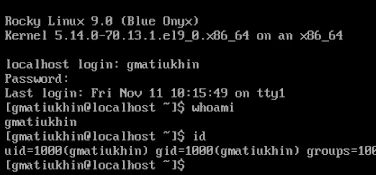
\includegraphics{1.png}\\
        \end{frame}
        \begin{frame}[plain]
        \item Используя комманду \texttt{su} для переключения к учетной записи \texttt{root}. При запросе пароля введите пароль пользователя \texttt{root}.\\Объясните информацию комманды \texttt{id}.
            \\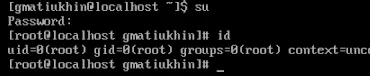
\includegraphics{2.png}\\
          \item Посмотрите в безопасном режиме файл \texttt{/etc/sudoers}
          \item Убедитесь, что в открытом файле присутствует строка\\ \texttt{wheel ALL=(ALL) ALL}
            \\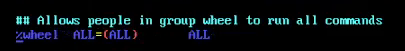
\includegraphics{3.png}\\
        \end{frame}
        \begin{frame}[plain]
        \item Создайте пользователя \texttt{alice}, входящего в группу \texttt{wheel}
        \item Убедитесь, что пользователь \texttt{alice} добавлен в группу \texttt{wheel}, введя \texttt{id alice}
          \\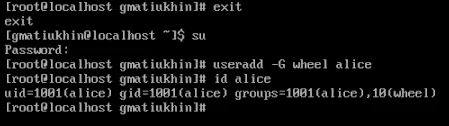
\includegraphics{4.png}\\
        \end{frame}
        \begin{frame}[plain]
        \item Задайте пароль для пользователя \texttt{alice}
        \item Переключитесь на учетную запись пользователя \texttt{alice}
        \item Создайте пользователя \texttt{bob}
        \item Установите пароль для пользователя \texttt{bob}
          \\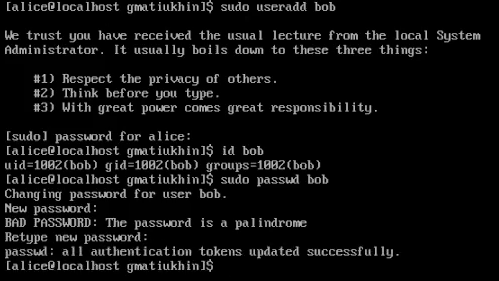
\includegraphics{5.png}\\
        \end{frame}
      \end{enumerate}
    \subsection{Создание учетных записей пользователей}
      \begin{enumerate}
        \begin{frame}[plain]
        \frametitle{Создание учетных записей пользователей}
        \item Перелючитесь в терминале на учетную запись пользователя \texttt{root}:
        \item Откройте файл конфигурации \texttt{/etc/login.defs} для редактирования.\\
          Убедитесь, что параметр \texttt{CREATE\_HOME} установлен в значение \texttt{yes}\\
          Установите параметр \texttt{USERGROUPS\_ENAB} в значение \texttt{no}
          \\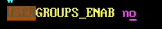
\includegraphics{6.png}
          \\\includegraphics{6\_1.png}\
        \end{frame}
        \begin{frame}[plain]
        \item Перейдите в каталог \texttt{/etc/skel/}, создайте каталоги \texttt{Pictures} и \texttt{Documents}
          \\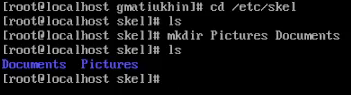
\includegraphics{7.png}\\
        \end{frame}
        \begin{frame}[plain]
        \item Измените содержимое файла \texttt{~/.bashrc}, добавив строку:\\
          \texttt{export EDITOR=/usr/bin/vim}
          \\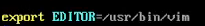
\includegraphics{8.png}\\
        \end{frame}
        \begin{frame}[plain]
        \item Используя утилиту \texttt{useradd}, создайте пользователя \texttt{carol}
        \item Установите пароль для пользователя \texttt{carol}
        \item Посмотрите информацию о пользователе \texttt{carol}
          \\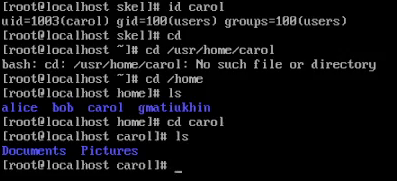
\includegraphics{9.png}\\
        \item Измените свойства пароля пользователя \texttt{carol} следующим образом
          \\
\includegraphics{10.png}\\
        \end{frame}
        \begin{frame}[plain]
        \item Создайте еще несколько пользователей используя скрипт
          \\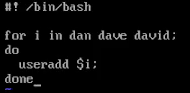
\includegraphics{11.png}\\
        \end{frame}
        \begin{frame}[plain]
        \item Убедитесь, что идентификатор \texttt{alice} существует во всех трех файлах
        \item Убедитесь, что идентиыикатор \texttt{carol} существует не во всех трех файлах
          \\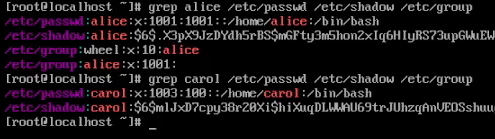
\includegraphics{12.png}\\
        \end{frame}
      \end{enumerate}
    \subsection{Работа с группами}
      \begin{enumerate}
        \begin{frame}[plain]
      \frametitle{Работа с группами}
        \item Находясь под учетной записью пользователя \texttt{root}, создайте группы \texttt{main} и \texttt{third}
        \item Используйте \texttt{usermod} для добавления пользователей \texttt{alice} и \texttt{bob} в группу \texttt{main}, а \texttt{carol}, \texttt{dan}, \texttt{dave} и \texttt{david} -- в группу \texttt{third}
          \\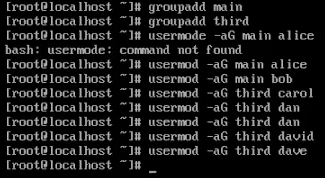
\includegraphics{13.png}\\
        \end{frame}
        \begin{frame}[plain]
        \item Убедитесь, что пользователь \texttt{carol} правильно добавлен в группу \texttt{third}.\\
          Опредеделите, в какие вторичные группы входит \texttt{carol}.
          \\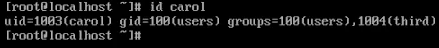
\includegraphics{14.png}\\
        \end{frame}
      \end{enumerate}
  \section{Вывод}
    \begin{frame}[plain]
      \frametitle{Вывод}
      В ходе выполнения данной работы я получил представление о работе с учётными записями пользователей и группами пользователей в операционной системе типа Linux
    \end{frame}
\end{document}
